% Options for packages loaded elsewhere
\PassOptionsToPackage{unicode,citecolor=black}{hyperref}
\PassOptionsToPackage{hyphens}{url}
\PassOptionsToPackage{dvipsnames,svgnames,x11names}{xcolor}
%
\documentclass[
  authoryear,
  preprint,
  3p]{elsarticle}

\usepackage{amsmath,amssymb}
\usepackage{iftex}
\ifPDFTeX
  \usepackage[T1]{fontenc}
  \usepackage[utf8]{inputenc}
  \usepackage{textcomp} % provide euro and other symbols
\else % if luatex or xetex
  \usepackage{unicode-math}
  \defaultfontfeatures{Scale=MatchLowercase}
  \defaultfontfeatures[\rmfamily]{Ligatures=TeX,Scale=1}
\fi
\usepackage{lmodern}
\ifPDFTeX\else  
    % xetex/luatex font selection
\fi
% Use upquote if available, for straight quotes in verbatim environments
\IfFileExists{upquote.sty}{\usepackage{upquote}}{}
\IfFileExists{microtype.sty}{% use microtype if available
  \usepackage[]{microtype}
  \UseMicrotypeSet[protrusion]{basicmath} % disable protrusion for tt fonts
}{}
\makeatletter
\@ifundefined{KOMAClassName}{% if non-KOMA class
  \IfFileExists{parskip.sty}{%
    \usepackage{parskip}
  }{% else
    \setlength{\parindent}{0pt}
    \setlength{\parskip}{6pt plus 2pt minus 1pt}}
}{% if KOMA class
  \KOMAoptions{parskip=half}}
\makeatother
\usepackage{xcolor}
\setlength{\emergencystretch}{3em} % prevent overfull lines
\setcounter{secnumdepth}{5}
% Make \paragraph and \subparagraph free-standing
\ifx\paragraph\undefined\else
  \let\oldparagraph\paragraph
  \renewcommand{\paragraph}[1]{\oldparagraph{#1}\mbox{}}
\fi
\ifx\subparagraph\undefined\else
  \let\oldsubparagraph\subparagraph
  \renewcommand{\subparagraph}[1]{\oldsubparagraph{#1}\mbox{}}
\fi


\providecommand{\tightlist}{%
  \setlength{\itemsep}{0pt}\setlength{\parskip}{0pt}}\usepackage{longtable,booktabs,array}
\usepackage{calc} % for calculating minipage widths
% Correct order of tables after \paragraph or \subparagraph
\usepackage{etoolbox}
\makeatletter
\patchcmd\longtable{\par}{\if@noskipsec\mbox{}\fi\par}{}{}
\makeatother
% Allow footnotes in longtable head/foot
\IfFileExists{footnotehyper.sty}{\usepackage{footnotehyper}}{\usepackage{footnote}}
\makesavenoteenv{longtable}
\usepackage{graphicx}
\makeatletter
\def\maxwidth{\ifdim\Gin@nat@width>\linewidth\linewidth\else\Gin@nat@width\fi}
\def\maxheight{\ifdim\Gin@nat@height>\textheight\textheight\else\Gin@nat@height\fi}
\makeatother
% Scale images if necessary, so that they will not overflow the page
% margins by default, and it is still possible to overwrite the defaults
% using explicit options in \includegraphics[width, height, ...]{}
\setkeys{Gin}{width=\maxwidth,height=\maxheight,keepaspectratio}
% Set default figure placement to htbp
\makeatletter
\def\fps@figure{htbp}
\makeatother

\usepackage{gensymb}
\makeatletter
\@ifpackageloaded{caption}{}{\usepackage{caption}}
\AtBeginDocument{%
\ifdefined\contentsname
  \renewcommand*\contentsname{Table of contents}
\else
  \newcommand\contentsname{Table of contents}
\fi
\ifdefined\listfigurename
  \renewcommand*\listfigurename{List of Figures}
\else
  \newcommand\listfigurename{List of Figures}
\fi
\ifdefined\listtablename
  \renewcommand*\listtablename{List of Tables}
\else
  \newcommand\listtablename{List of Tables}
\fi
\ifdefined\figurename
  \renewcommand*\figurename{Figure}
\else
  \newcommand\figurename{Figure}
\fi
\ifdefined\tablename
  \renewcommand*\tablename{Table}
\else
  \newcommand\tablename{Table}
\fi
}
\@ifpackageloaded{float}{}{\usepackage{float}}
\floatstyle{ruled}
\@ifundefined{c@chapter}{\newfloat{codelisting}{h}{lop}}{\newfloat{codelisting}{h}{lop}[chapter]}
\floatname{codelisting}{Listing}
\newcommand*\listoflistings{\listof{codelisting}{List of Listings}}
\makeatother
\makeatletter
\makeatother
\makeatletter
\@ifpackageloaded{caption}{}{\usepackage{caption}}
\@ifpackageloaded{subcaption}{}{\usepackage{subcaption}}
\makeatother
\makeatletter
\@ifpackageloaded{sidenotes}{}{\usepackage{sidenotes}}
\@ifpackageloaded{marginnote}{}{\usepackage{marginnote}}
\makeatother
\journal{PsyArxiv}
\ifLuaTeX
  \usepackage{selnolig}  % disable illegal ligatures
\fi
\usepackage[]{natbib}
\bibliographystyle{elsarticle-harv}
\IfFileExists{bookmark.sty}{\usepackage{bookmark}}{\usepackage{hyperref}}
\IfFileExists{xurl.sty}{\usepackage{xurl}}{} % add URL line breaks if available
\urlstyle{same} % disable monospaced font for URLs
\hypersetup{
  pdftitle={Supplementary Material (A) - Procedure for testing and adjusting translations of the Soundscape (quasi-)Circumplex Model},
  pdfauthor={Andrew Mitchell; Francesco Aletta},
  colorlinks=true,
  linkcolor={blue},
  filecolor={Maroon},
  citecolor={Blue},
  urlcolor={Blue},
  pdfcreator={LaTeX via pandoc}}

\setlength{\parindent}{6pt}
\begin{document}

\begin{frontmatter}
\title{Supplementary Material (A) - Procedure for testing and adjusting
translations of the Soundscape (quasi-)Circumplex Model}
\author[1]{Andrew Mitchell%
\corref{cor1}%
}
 \ead{andrew.mitchell.18@ucl.ac.uk} 
\author[1]{Francesco Aletta%
%
}
 \ead{f.aletta@ucl.ac.uk} 

\affiliation[1]{organization={University College London, Institute for
Environmental Design and Engineering},addressline={Central House, 14
Upper Woburn Place},city={London},postcode={WC1H 0NN},postcodesep={}}

\cortext[cor1]{Corresponding author}


        
\begin{abstract}
In depth description for the procedure developed for the paper:
``Soundscape descriptors in eighteen languages: translation and
validation through listening experiments
\end{abstract}





\end{frontmatter}
    \section{Introduction}\label{introduction}

In this analysis, we aim to test the circumplex structure of various
soundscape survey translations. The circumplex model is a powerful tool
in psychology, often used to visualize and interpret complex
multivariate data. In order to enable its use across many contexts,
cultures, and languages, its necessary to validate the structure of the
circumplex items. The goal of validated translations is to ensure that
the circumplex structure is maintained across translations, allowing for
cross-cultural comparisons.

\subsection{Defining the circumplex
model}\label{defining-the-circumplex-model}

The concept of the psychometric circumplex model, first introduced by
\citet{Guttman1954new}, revolves around the idea of a circular
relationship among variables. This circular relationship can be seen by
identifying certain correlation patterns within the correlation matrix
among variables, when appropriately ordered
\citep{Browne1992Circumplex}. In the case of the circular structure, the
strength of the correlation coefficients in the matrix decreases as you
move away from the diagonal, and then increases again as you move
towards the opposite diagonal. This pattern of correlations can be seen
in Table~\ref{tbl-circumplex}.

\begin{longtable}[]{@{}
  >{\raggedright\arraybackslash}p{(\columnwidth - 16\tabcolsep) * \real{0.0714}}
  >{\raggedright\arraybackslash}p{(\columnwidth - 16\tabcolsep) * \real{0.1122}}
  >{\raggedright\arraybackslash}p{(\columnwidth - 16\tabcolsep) * \real{0.1122}}
  >{\raggedright\arraybackslash}p{(\columnwidth - 16\tabcolsep) * \real{0.1122}}
  >{\raggedright\arraybackslash}p{(\columnwidth - 16\tabcolsep) * \real{0.1122}}
  >{\raggedright\arraybackslash}p{(\columnwidth - 16\tabcolsep) * \real{0.1122}}
  >{\raggedright\arraybackslash}p{(\columnwidth - 16\tabcolsep) * \real{0.1122}}
  >{\raggedright\arraybackslash}p{(\columnwidth - 16\tabcolsep) * \real{0.1122}}
  >{\raggedright\arraybackslash}p{(\columnwidth - 16\tabcolsep) * \real{0.0714}}@{}}
\caption{Theoretical pattern of the correlation matrix corresponding to
a circular structure. \(\rho_1 > \rho_2 > \rho_3 > \rho_4\)
\citep{Gurtman2000Interpersonal}.}\label{tbl-circumplex}\tabularnewline
\toprule\noalign{}
\begin{minipage}[b]{\linewidth}\raggedright
\end{minipage} & \begin{minipage}[b]{\linewidth}\raggedright
V1
\end{minipage} & \begin{minipage}[b]{\linewidth}\raggedright
V2
\end{minipage} & \begin{minipage}[b]{\linewidth}\raggedright
V3
\end{minipage} & \begin{minipage}[b]{\linewidth}\raggedright
V4
\end{minipage} & \begin{minipage}[b]{\linewidth}\raggedright
V5
\end{minipage} & \begin{minipage}[b]{\linewidth}\raggedright
V6
\end{minipage} & \begin{minipage}[b]{\linewidth}\raggedright
V7
\end{minipage} & \begin{minipage}[b]{\linewidth}\raggedright
V8
\end{minipage} \\
\midrule\noalign{}
\endfirsthead
\toprule\noalign{}
\begin{minipage}[b]{\linewidth}\raggedright
\end{minipage} & \begin{minipage}[b]{\linewidth}\raggedright
V1
\end{minipage} & \begin{minipage}[b]{\linewidth}\raggedright
V2
\end{minipage} & \begin{minipage}[b]{\linewidth}\raggedright
V3
\end{minipage} & \begin{minipage}[b]{\linewidth}\raggedright
V4
\end{minipage} & \begin{minipage}[b]{\linewidth}\raggedright
V5
\end{minipage} & \begin{minipage}[b]{\linewidth}\raggedright
V6
\end{minipage} & \begin{minipage}[b]{\linewidth}\raggedright
V7
\end{minipage} & \begin{minipage}[b]{\linewidth}\raggedright
V8
\end{minipage} \\
\midrule\noalign{}
\endhead
\bottomrule\noalign{}
\endlastfoot
V1 & 1 & & & & & & & \\
V2 & \(\rho_1\) & 1 & & & & & & \\
V3 & \(\rho_2\) & \(\rho_1\) & 1 & & & & & \\
V4 & \(\rho_3\) & \(\rho_2\) & \(\rho_1\) & 1 & & & & \\
V5 & \(\rho_4\) & \(\rho_3\) & \(\rho_2\) & \(\rho_1\) & 1 & & & \\
V6 & \(\rho_3\) & \(\rho_4\) & \(\rho_3\) & \(\rho_2\) & \(\rho_1\) & 1
& & \\
V7 & \(\rho_2\) & \(\rho_3\) & \(\rho_4\) & \(\rho_3\) & \(\rho_2\) &
\(\rho_1\) & 1 & \\
V8 & \(\rho_1\) & \(\rho_2\) & \(\rho_3\) & \(\rho_4\) & \(\rho_3\) &
\(\rho_2\) & \(\rho_1\) & 1 \\
\end{longtable}

This pattern of the corrrelation matrix indicates that the variables are
ordered in a circular fashion, with the strongest correlations between
adjacent variables, and the weakest correlations between variables that
are furthest apart. It also means that the correlations between these
variables follow a pattern that increases and decreases in a way that
resembles a cosine wave, as explained by \citet{Yik2004Relationship} and
\citet{Grassi2010CircE}. This circular arrangement of the variables can
be tested using a method proposed by \citet{Rounds2000Tinsley}.

Browne further expanded on the circumplex model in 1992 and 1995 by
differentiating between equal spacing and equal communality (or radii)
constraints. Browne described four variations of circumplex models,
which include three types of quasi-circumplex models and one circulant
model. These variations include the unconstrained or loosely ordered
quasi-circumplex, the equal spacing quasi-circumplex, the equal
communality quasi-circumplex, and the circulant model that maintains
both equal spacing and equal communality.

In certain instances, the rigidity of a circumplex may be relaxed,
leading to the concept of a quasi-circumplex. The term ``quasi'' implies
a departure from strict adherence to even spacing and equal communality,
allowing for some flexibility in the arrangement of variables. This
flexibility is often necessary in order to accommodate the complexity of
psychological constructs, which may not always fit neatly into a rigid
circular structure. It refers to any graphical or conceptual
representation where variables or dimensions are organized in a circular
or circular-like manner. This umbrella term recognizes the spectrum of
circular models, acknowledging variations in the spacing, organization,
and relationships among variables.

As researchers delve into the intricacies of psychological spaces, the
choice between a strict circumplex, a quasi-circumplex, or a more
general circular structure becomes crucial. These models play a pivotal
role in visualizing and understanding the complex interplay of
variables, offering researchers nuanced frameworks to explore and
interpret their data.

As described by \citet{Rogoza2021three}:

\begin{quote}
The circumplex model can be defined through the terms of: 1) the
possibility to locate variables differentiated in the model in the
two-dimensional space with 2) equal spacing (i.e.~same distance between
variables within the model around circumplex) and 3) equal communality
(i.e.~same distance between variables from the middle of the circle)
\citep[\citet{Pincus2003Interpersonal}]{Gurtman1994differentiating}. On
the basis of these criteria, one could differentiate four models,
depicted on Fig. 1: a circular one (less restrictive Model 1),
quasi-circumplex (Model 2 and 3), and circumplex (most restrictive Model
4).
\end{quote}



\subsection{Locating external variables within circumplex
models}\label{locating-external-variables-within-circumplex-models}

Once the general circumplex structure is tested, it is possible to
investigate the likelihood to locate an external variable (e.g.,
psychoacoustic loudness, N) within the empirical circumplex. The
circumplex model provides a precise framework for predicting the
relationships between an external variable and all circumplex variables.
The Structural Summary Method (SSM) yields several key estimations,
including: Model fit (R2), which assesses how well the observed
sinusoidal curve aligns with the cosine function, indicating the
goodness of fit. Elevation, representing the average correlation between
an external variable and all circumplex variables. Amplitude (vector
length), measuring the distance from the mean of the external variable's
correlation to its peak correlation with circumplex variables. This
value signifies the uniqueness of the profile, indicating whether it is
prominently associated with a specific circumplex variable or equally
related to all. Angular displacement, denoting the angle at which the
profile reaches its maximum point, indicating the empirical location of
the variable within the circumplex as observed in the data. The
Structural Summary Method (SSM) is a technique used to summarize
correlation patterns among measurement scores that are hypothesized to
conform to a circumplex structure (Rogoza, Cieciuch, \& Strus, 2021).
SSM aims to fit a sinusoidal curve to data points (qi) based on their
nominal angular positions (θi). This is achieved by optimizing the
parameters for elevation (e), amplitude (i), and displacement (d).
Mathematically, these parameters are used to model the correlational
information (qi) in equation 1: q\_i=e+α cos⁡〖(θ\_i-d)〗. (1) It is
essential to evaluate how well the sinusoidal curve aligns with the
cosine function by examining its goodness of fit, as indicated by the R2
value. If R2values fall below 0.70, it is advisable not to interpret the
remaining coefficients and to discontinue the process of locating
external variables. Conversely, R2 values exceeding 0.80 indicate a
strong fit. Additionally, it's worth mentioning that amplitude
estimates, reflecting the distinctiveness of the profile, and elevation
estimates, indicating the presence of a general factor, are considered
notable when they surpass 0.15.

The structure of the circumplex is key to determining where external
variables are located. Given differing angles and communalities, the
external variable can occupy different locations within the circumplex.
Revealing and validating the true structure of a particular circumplex
model is therefore key to reliably identifying correct location of
external variables within the circumplex space.

\subsection{Translating circumplex
instruments}\label{translating-circumplex-instruments}

Typically, circumplex scales are measured via a series of questions in a
survey instrument. These instruments are initially developed in one
language and the validity and structure of the instrument is tested in
that language. Often these instruments are directly translated into
other languages to enable their use in other countries. However, the
validity of the instrument in the new language is not guaranteed.
Changes in the correlation structure can be caused by errors in the
translation process, by semantic and linguistic differences between the
translated scales even given a valid translation, and by a lack of
generalisability of the circumplex instrument.

It is easy to see how errors in the translation process can lead to
changes in the correlation structure. For example, if a question is
mistranslated, then the responses to that question will not be
correlated with the responses to the other questions in the instrument.
Semantic and linguistic differences between the translated scales can
also lead to changes in the correlation structure. For example, if a
question is translated into a language where the concept does not exist
or cannot be easily expressed, then the responses to that question will
not be correlated with the responses to the other questions in the
instrument. Finally, it may be that even if the original instrument is
valid for e.g.~the English-speaking population, it may not be valid for
other populations due to cultural differences.

\subsubsection{Goals of translating a circumplex
instrument}\label{goals-of-translating-a-circumplex-instrument}

Two approaches could be taken when attempting to translate a survey
instrument. The first approach would attempt to achieve direct
concurrence with the original instrument, where each scale is directly
correlated with the corresponding scale from the original instrument. If
the circumplex structure is identical between the two languages, then
this approach would allow for the most direct comparison between the two
languages. However, if the circumplex structure is not identical between
the two languages, then this approach would lead to a loss of
information. The second approach would attempt to achieve the same
circumplex structure in the new language as in the original language.
This approach would allow for the most direct comparison between the two
languages.

In this second approach, identifying the differences in structure
between translations enable the process of locating an external variable
to be corrected for the differences in structure. Given that at minimum
a quasi-circumplex structure can be confirmed, then the deviations in
either the angles or communalities from the ideal circumplex structure
can be measured and accounted for. When this is done separately for the
origianl and translated instruments, then an external variable which has
the same theoretical location in both instruments should be located in
the same location in both corrected instruments.

This has an important impact on comparing results under the two
translations. If an external variable is theoretically located in a
single, fixed position in the circumplex space, locating it without
accounting for the differences in structure between the two translations
will lead to different locations in the two translations. The
interpretation of this result would then be that the external variable
is located in different positions in the two languages. However, if the
differences in structure are accounted for, then the external variable
should be located in the same position in both translations. By applying
the correction we can attempt to discover differences in the effect of
external variables, independent of the differences in structure between
the two translations.

\subsection{A test case: The Soundscape Circumplex Model
(SCM)}\label{a-test-case-the-soundscape-circumplex-model-scm}

In 2010, \citet{Axelsson2010principal} proposed a \emph{principle
components} model of soundscape perception. Due to its similarity to the
widely-studied Russell's circumplex model of affect
\citep{Russell1980circumplex}, Axelsson's principal component model is
often referred to as the Soundscape Circumplex Model (SCM) in soundscape
literature. The SCM and the Swedish Soundscape Quality Protocol (SSQP)
\citep{Axelsson2012Swedish} utilizing it quickly became the predominant
method of soundscape assessment in both scientific literature and
professional practice \citep{Aletta2023Adoption}, due to its ease of
use, interpretability, and, crucially, its ability to summarise the
complex interrelationships between soundscape descriptors within a
straightforward and familiar two-dimensional space. Togeter with a
similar principal component model in \citet{Cain2013development}, the
framework of the circumplex model of soundscape perception was
subsequently adapted into an integral part of the standardised protocols
for soundscape data collection, specifically in Method A of
\citet{ISO12913Part2}.

Currently, the soundscape community relies very heavily on the framework
proposed in \citet{ISO12913Part2}, both for theory development and for
procuring empirical evidence of the benefits of the soundscape approach,
in real life scenarios. In a recent systematic literature review,
\citet{Aletta2023Adoption} idenitified 254 scientific publications which
have referred to ISO 12913 since its publication in 2018, with 50 of
them appropriately making use of the data collection methods. Of those,
several papers included multiple studies, with 51 studies making use of
the SCM as recommended in the ISO standard. In addition, the SCM has
been used in many more studies without reference to the ISO standard
\citep{Engel2018Review}, and has been haphazardly translated into many
languages
\citep{Tarlao2016Comparing, Nagahata2019Examination, Tarlao2020Investigating, Aletta2019Exploringa}.

The Soundscape Circumplex Model (SCM) was developed in 2010 by
\citet{Axelsson2010principal} to describe the perception of ambient
sound environments. It has since been used in a number of studies to
describe the perception of soundscapes in different contexts and
cultures \citep{ISO12913Part2}. The SCM is composed of eight scales,
which closely resemble the eight scales of the Circumplex Model of
Affect \citep{Russell1980circumplex}. The 7 scales are arranged in two
bipolar dimensions, with pleasant-annoying along the x-axis (valence)
and eventful-uneventful along the y-axis (arousal). Arranged in a
circular pattern around the circumplex, beginning at 0 degrees and
moving counter-clockwise, the eight scales are: pleasant (0)

\section{A four step procedure for the analysis of circumplex
models}\label{a-four-step-procedure-for-the-analysis-of-circumplex-models}

In \citet{Rogoza2021three}, the authors propose a three-step procedure
for assessing circumplex models. The steps in this procedure are: 1)
``verify whether the analzed model is circumplex or not'' using
Structural Equation Modelling based on \citet{Browne1992Circumplex}'s
model; 2) ``test the possibility to locate an external variable within
empirical circumplex'' using the Structural Summary Method
\citep{Gurtman1994differentiating}; and 3) ``assess the extent of which
empirical locations are in congruence to the theoretical predictions
within the circumplex structure'' \citep{Rogoza2021three}.

We expand upon the three-step procedure proposed by
\citet{Rogoza2021three} and adapt it to the specific case of testing
multiple variations (i.e.~translations) of the same circumplex
instrument. The goals of this procedure are, for each translation, to
verify the quasi-circumplex structure of the instrument, to derive angle
corrections, and to test the congruence between the corrected circumplex
and the theoretical circumplex structure. We do this by first adding an
initial step to incorporate \citet{Rounds2000Tinsley}'s test of the
circular ordering of the scales to confirm that the order of the scales
is maintained across translations. We then follow the same three steps
as \citet{Rogoza2021three}, but we adapt the third step to test the
congruence between the circumplex structure of the original instrument
and the circumplex structure of the translated instruments and to allow
for adjustments to be made by extracting adjusted angles from the SEM
step.

\subsection{Step 1: Confirm the circular ordering of the circumplex
scales}\label{step-1-confirm-the-circular-ordering-of-the-circumplex-scales}

In line with the procedure taken in \citet{Gurtman2000Interpersonal}, we
begin by confirming the circular ordering of the circumplex scales. This
test, developed by \citet{Rounds2000Tinsley}, the test of the circular
order model involves comparing the obtained order relations for a set of
scales against their hypothesized order given a certain circular model.
This test is applied in order to ensure that the process of translation
has not altered the order of the scales and so the test is applied
against the order of the scales in the original instrument. The test is
applied to each translation separately, and the results are compiled
into a single table.

The index used for this test is \citet{Hubert1987Evaluating}'s
correspondence index (CI). This offers a descriptive measure reflecting
the degree to which the model's ordered predictions align with a
specific sample matrix. The metric is calculated as the proportion of
predictions met minus the proportion violated, yielding a range from 1.0
(indicating complete prediction fulfillment) to -1.0 (indicating all
predictions contradicted). In alignment with the methodology outlined by
Tracey et al. \citep{Tracey1997RANDALL}, we applied a randomization test
to the hypothesized order relations \citep{Hubert1987Evaluating},
producing an exact probability, determining the likelihood of achieving
the observed model fit in relation to all potential permutations of the
matrix. The index thresholds for this test are: a p-value \textless{}
0.05 and a CI \textgreater{} 0.70.

\subsection{Step 2: Confirm the quasi-circumplex structure of the
circumplex
scales}\label{step-2-confirm-the-quasi-circumplex-structure-of-the-circumplex-scales}

We confirm the structure of the circumplex instrument by applying
\citet{Browne1992Circumplex}'s circular stochastic process model with a
Fourier series correlation function. This model represents a
non-standard Structural Equation Model (SEM) specifically tailored to
testing circumplex structures which allows a researcher to examine the
extent to which the underlying structure of a sample correlation matrix
conforms to a circumplex pattern. The four model variations
(unconstrained circular, equal spacing quasi-circumplex,
equal-communality quasi-circumplex, and strict circumplex with equal
spacing and communality) can each be investigated using this model. For
the unconstrained and quasi-circumplex models, Brownen's model allows
for the estimation of the angles and communalities of the circumplex
scales. From these results for the quasi-circumplex models, we can
derive the corrected angles (or communalities) for each translation,
which can be used in the next step of the analysis.

This model is implemented in the CircE package \citep{Grassi2010CircE}
for R \citep{RCT2018R}. The model is applied to each translation
separately, testing each of the four model variations, and the results
are compiled into a single table. CircE provides a suite suite of SEM
fit indices, which are statistical measures used to evaluate the
goodness of fit of the models. For this study, we use the following fit
indices: Comparative Fit Index (CFI), Goodness of Fit Index (GFI), and
Standardized Root Mean Square Residual (SRMR), summarised with their
respective thresholds in Table~\ref{tbl-indices}.

Readers might note that these indices differ slightly from those used by
Rogoza et al., most notably the exclusion of the Root Mean Square Error
of Approximation (RMSEA), a commonly used metric. RMSEA was excluded
from the analysis on the basis of both Rogoza's own critiques\footnote{``it
  is worth noting that the RMSEA may not be best suited to evaluate
  circumplex models. It becomes biased in the case of high correlations
  between proximal variables, as found in circumplex models, and should
  be interpreted with caution.'' \citep{Rogoza2021three}} and recent
warnings from \citet{West2022Handbook}.

\begin{longtable}[]{@{}
  >{\raggedright\arraybackslash}p{(\columnwidth - 4\tabcolsep) * \real{0.5106}}
  >{\centering\arraybackslash}p{(\columnwidth - 4\tabcolsep) * \real{0.1809}}
  >{\centering\arraybackslash}p{(\columnwidth - 4\tabcolsep) * \real{0.2979}}@{}}
\caption{Fit indices and thresholds, including the reference from which
the threshold is derived.}\label{tbl-indices}\tabularnewline
\toprule\noalign{}
\begin{minipage}[b]{\linewidth}\raggedright
\textbf{Fit Index}
\end{minipage} & \begin{minipage}[b]{\linewidth}\centering
\textbf{Threshold}
\end{minipage} & \begin{minipage}[b]{\linewidth}\centering
\textbf{Reference}
\end{minipage} \\
\midrule\noalign{}
\endfirsthead
\toprule\noalign{}
\begin{minipage}[b]{\linewidth}\raggedright
\textbf{Fit Index}
\end{minipage} & \begin{minipage}[b]{\linewidth}\centering
\textbf{Threshold}
\end{minipage} & \begin{minipage}[b]{\linewidth}\centering
\textbf{Reference}
\end{minipage} \\
\midrule\noalign{}
\endhead
\bottomrule\noalign{}
\endlastfoot
Correspondence Index (CI) & p \textless{} 0.05,

CI \textgreater{} 0.70 & \citet{Gurtman2000Interpersonal} \\
Comparative Fit Index (CFI) & \emph{0.92} &
\citet{Moshona2023Optimization} \\
Goodness of Fit Index (GFI) & \emph{0.90} & \citet{Rogoza2021three} \\
Standardized Root Mean Square Residual (SRMR) & \emph{0.08} &
\citet{Moshona2023Optimization}

\citet{Tarlao2020Investigating} \\
\end{longtable}

Once each of the model variations are assessed against the above fit
indices, we can determine whether that model variation is a good fit for
the data. If the strict circumplex model meets the fit thresholds across
the translations tested, then the procedure can be continued and no
adjustment will be needed. If, however, the structure of some or all of
the translations are found to have a quasi-circumplex structure, then
adjustments will need to be derived and applied to ensure
cross-comparability between the translated instruments. If the model
variation for the equal-communality model (where the angles are allowed
to vary) is a good fit for the data, then we can use the derived angles
from CircE as adjustments to the circumplex structure.

Importantly, this table also reports the derived angles for each scale
for the unconstrained and Equal comm. models. These angles will be
carried over and used in the next stage of the analysis, where we will
validate the survey instrument by correlating the survey responses with
the acoustic indices using the Structural Summary Method (SSM).

\subsection{Step 3: Locate the full dataset circumplex scales within
each language's circumplex
space}\label{step-3-locate-the-full-dataset-circumplex-scales-within-each-languages-circumplex-space}

Once the general circumplex structure is tested, it is possible to
investigate the likelihood to locate an external variable (this could be
an objective feature such as sound level dB or it could be another
perceptual or psychometric variable such as tranquility) within the
empirical circumplex. The circumplex model provides a precise framework
for predicting the relationships between an external variable and all
circumplex variables. The Structural Summary Method (SSM) is a technique
used to summarize correlation patterns among measurement scores that are
hypothesized to conform to a circumplex structure
\citep{Rogoza2021three}. SSM aims to fit a sinusoidal curve to data
points (\(q_i\)) based on their nominal angular positions
(\(\theta_i\)). This is achieved by optimizing the parameters for
elevation (\(e\)), amplitude (\(i\)), and displacement (\(d\)).
Mathematically, these parameters are used to model the correlational
information (\(q_i\)) in Equation~\ref{eq-ssm}:

\begin{equation}\phantomsection\label{eq-ssm}{
q_i = e + \alpha cos(\theta_i - d)
}\end{equation}

SSM analysis yields several key estimations, including:

\begin{itemize}
\tightlist
\item
  Model fit (R2), which assesses how well the observed sinusoidal curve
  aligns with the cosine function, indicating the goodness of fit.
\item
  Elevation, representing the average correlation between an external
  variable and all circumplex variables.
\item
  Amplitude (vector length), measuring the distance from the mean of the
  external variable's correlation to its peak correlation with
  circumplex variables. This value signifies the uniqueness of the
  profile, indicating whether it is prominently associated with a
  specific circumplex variable or equally related to all.
\item
  Angular displacement, denoting the angle at which the profile reaches
  its maximum point, indicating the empirical location of the variable
  within the circumplex as observed in the data.
\end{itemize}

\begin{quote}
It is essential to evaluate how well the sinusoidal curve aligns with
the cosine function by examining its goodness of fit, as indicated by
the \(R^2\) value. If \(R^2\) values fall below 0.70, it is advisable
not to interpret the remaining coefficients and to discontinue the
process of locating external variables. Conversely, \(R^2\) values
exceeding 0.80 indicate a strong fit. Additionally, it's worth
mentioning that amplitude estimates, reflecting the distinctiveness of
the profile, and elevation estimates, indicating the presence of a
general factor, are considered notable when they surpass 0.15.
\end{quote}

As described in \citet{Rogoza2021three}, Step Two involves testing
whether external variables can be located within the circumplex.

Because we have derived new angles in the SEM step, we use these
`adjusted' angles for calculating the SSM parameters.

In order to determine whether the language circumplexes can adequately
allow an external variable to be located, we use the following criteria:

\begin{itemize}
\tightlist
\item
  \(R^2\) \textgreater{} 0.8
\item
  amplitude \textgreater{} .15
\end{itemize}

These indices are based on the criteria used by \citet{Rogoza2021three},
however we use an increased criterion of \(R^2 > 0.9\) since we have a
prior expectation that the circumplex variables should fit very well
within each translation's circumplex.

\subsection{Step 4: Accurately locating circumplex items within each
language}\label{step-4-accurately-locating-circumplex-items-within-each-language}

The final step of \citet{Rogoza2021three} 's three step procedure is to
test the congruence between the empirical locations and theoretical
expectations within the circumplex structure. In the case of the
soundscape circumplex and our SATP data, we don't have an external
variable with a defined theoretical location within the circumplex - for
instance loudness does not have a defined location within the circumplex
where it is expected to be located.

Taking inspiration from \citet{Yik2004Relationship}, we propose to use
the circumplex structure of the soundscape survey itself as the
theoretical expectation. \citet{Yik2004Relationship} proposes that one
circumplex can be located within another by calculating the SSM
correlation between each of the scales of the reference circumplex and
the test circumplex. In this way, each scale of the reference circumplex
can be located within the test circumplex, and we can test whether these
empirical locations meet our expectations.

The process to do this is as follows:

\begin{enumerate}
\def\labelenumi{\arabic{enumi}.}
\tightlist
\item
  For both the reference and test circumplex, calculate the mean value
  of each scale for each recording.
\item
  Calculate the SSM correlation between each scale of the reference
  circumplex and the test circumplex, in our case using the corrected
  angles.
\item
  Test the congruence betwen the empirical locations and theoretical
  expectations using the Procrustes congruence test
  \citep{Rogoza2021three}.
\end{enumerate}

We will be using the full dataset as the reference set and the data from
each translation as the test set. This effectively means that we are
testing whether each translation is able to locate the circumplex
structure of the soundscape survey, consistently across all languages.

This aligns with the overall goal of our process of allowing data
(i.e.~the circumplex coordinate) from different languages to be directly
compared, by correcting for the differences in the circumplex structure
between languages.

\subsubsection{Congruence}\label{congruence}

What \citet{Rogoza2021three} (and Orthosim) refer to as Tucker's
Congruence Coefficient is also commonly referred to as the cosine
similarity (see the
\href{https://tensorly.org/stable/modules/generated/tensorly.metrics.factors.congruence_coefficient.html}{Tensorly
documentation}). We therefore use the sklearn implementation of cosine
similarity to calculate the congruence between the empirical locations
and theoretical expectations. This produces a matrix of cosine
similarity values, which we then use to calculate the mean congruence,
to match the model congruence from \citet{Rogoza2021three}.

\subsubsection{Procrustes}\label{procrustes}

However, it appears that, despite \citet{Rogoza2021three} 's
description, this method is not actually based on a Procrustes analysis.
The equivalent distance metric from a Procrustes method would be the
rotational-based Procrustes distance, i.e.~the squared Froebenius norm
of the difference between the two orthogonal matrices. See
\citet{Andreella2023Procrustes}:

\begin{quote}
Instead, the second distance exploits the orthogonal matrix parameters
solution of the Procrustes problem. The rotational-based distance
computes the squared Frobenius distance between these estimated
orthogonal matrices. As we will see, this metric measures the level of
dissimilarity/similarity in orientation between matrices/subjects before
functional alignment.
\end{quote}

Based on the proof given in \citet{Baktiar2015symmetrical}, given that
the input matrices are scaled (i.e.~\texttt{rotational(scale=True)}),
then the Procrustes distance is a true distance measure which obeys
\(0 < p(X, Y) < 1\) \citep[322]{Bakhtiar2015symmetrical}. Therefore we
can convert the Procrustes distance to a similarity measure by
subtracting it from 1.

\section{Results}\label{results}

\subsection{Step 1: Confirm the circular ordering of the circumplex
scales}\label{step-1-confirm-the-circular-ordering-of-the-circumplex-scales-1}

The results of the circular ordering test are shown in
Table~\ref{tbl-circular-order}. The following translations were not
confirmed to have a circular ordering of their scales which matches the
theoretical order: `zsm' and `vie'. They are therefore excluded from the
following steps of the analysis.

\begin{longtable}[]{@{}ccccccc@{}}

\caption{\label{tbl-circular-order}Results of the Circular Order
analysis of the SATP dataset.}

\tabularnewline

\toprule\noalign{}
mat & pred & met & tie & CI & p & description \\
\midrule\noalign{}
\endhead
\bottomrule\noalign{}
\endlastfoot
1 & 288 & 283 & 0 & 0.965 & 0.000 & SATP \\
2 & 288 & 272 & 0 & 0.889 & 0.000 & arb \\
3 & 288 & 262 & 0 & 0.819 & 0.000 & cmn \\
4 & 288 & 284 & 0 & 0.972 & 0.000 & deu \\
5 & 288 & 276 & 0 & 0.917 & 0.000 & ell \\
6 & 288 & 286 & 0 & 0.986 & 0.000 & eng \\
7 & 288 & 278 & 0 & 0.931 & 0.000 & fra \\
8 & 288 & 268 & 0 & 0.861 & 0.000 & hrv \\
9 & 288 & 255 & 0 & 0.771 & 0.000 & ind \\
10 & 288 & 275 & 0 & 0.910 & 0.000 & ita \\
11 & 288 & 264 & 0 & 0.833 & 0.000 & jpn \\
12 & 288 & 262 & 0 & 0.819 & 0.000 & kor \\
13 & 288 & 261 & 0 & 0.812 & 0.000 & nld \\
14 & 288 & 254 & 0 & 0.764 & 0.000 & por \\
15 & 288 & 283 & 0 & 0.965 & 0.000 & spa \\
16 & 288 & 284 & 0 & 0.972 & 0.000 & swe \\
17 & 288 & 261 & 0 & 0.812 & 0.000 & tur \\
18 & 288 & 244 & 0 & 0.694 & 0.002 & vie \\
19 & 288 & 241 & 0 & 0.674 & 0.002 & zsm \\

\end{longtable}

\subsection{Step 2: Confirm the quasi-circumplex structure of the
circumplex
scales}\label{step-2-confirm-the-quasi-circumplex-structure-of-the-circumplex-scales-1}

The results of the SEM model fit for the equal-communality
quasi-circumplex structures are shown in Table~\ref{tbl-sem-res}.

\begin{longtable}[]{@{}llllllllll@{}}

\caption{\label{tbl-sem-res}SEM fit results}

\tabularnewline

\toprule\noalign{}
& Language & Model Type & n & m & CFI & GFI & SRMR & Score & passing \\
\midrule\noalign{}
\endhead
\bottomrule\noalign{}
\endlastfoot
1 & eng & Equal comm. & 864 & 3 & 0.93 & 0.91 & 0.05 & 3 & Pass \\
5 & arb & Equal comm. & 809 & 3 & 0.97 & 0.97 & 0.04 & 3 & Pass \\
9 & cmn & Equal comm. & 1832 & 3 & 0.96 & 0.95 & 0.04 & 3 & Pass \\
13 & deu & Equal comm. & 810 & 3 & 0.94 & 0.92 & 0.06 & 3 & Pass \\
17 & ell & Equal comm. & 810 & 3 & 0.93 & 0.93 & 0.08 & 3 & Pass \\
25 & hrv & Equal comm. & 864 & 3 & 0.95 & 0.93 & 0.06 & 3 & Pass \\
29 & ind & Equal comm. & 891 & 3 & 0.93 & 0.92 & 0.08 & 3 & Pass \\
33 & ita & Equal comm. & 810 & 3 & 0.94 & 0.93 & 0.07 & 3 & Pass \\
41 & kor & Equal comm. & 810 & 3 & 0.95 & 0.94 & 0.08 & 3 & Pass \\
45 & nld & Equal comm. & 864 & 3 & 0.97 & 0.94 & 0.06 & 3 & Pass \\
53 & spa & Equal comm. & 1647 & 3 & 0.92 & 0.91 & 0.06 & 3 & Pass \\
57 & swe & Equal comm. & 945 & 3 & 0.94 & 0.92 & 0.05 & 3 & Pass \\
61 & tur & Equal comm. & 918 & 3 & 0.93 & 0.92 & 0.08 & 3 & Pass \\
21 & fra & Equal comm. & 891 & 3 & 0.92 & 0.91 & 0.10 & 2 & Fail \\
49 & por & Equal comm. & 1890 & 3 & 0.92 & 0.92 & 0.09 & 2 & Fail \\
37 & jpn & Equal comm. & 917 & 3 & 0.89 & 0.90 & 0.09 & 1 & Fail \\

\end{longtable}

Of the remaining 16 languages considered, all but 3 pass the fit indices
thresholds. The three which do not achieve the required performance are
`fra', `por', and `jpn'. These are excluded from the following steps of
the analysis.

\subsection{Step 3: Locate the full dataset circumplex scales within
each language's circumplex
space}\label{step-3-locate-the-full-dataset-circumplex-scales-within-each-languages-circumplex-space-1}

Figure~\ref{fig-profile-plots} demonstrates the SSM process for locating
each of the circumplex scales within the circumplex space of the `cmn'
translation. These profile plots show the correlation between the
circumplex scales and the external variable (in this case, each of the
general attributes) as a function of the angle of the circumplex scale.
The SSM model fits a sinusoidal curve to the data points, and the
parameters of this curve are used to determine the location of the
circumplex scale within the circumplex space. These plots show clearly
how adjusting the angles of the circumplex scales can improve the fit of
the sinusoidal curve to the data points.

\begin{figure}

\begin{minipage}[t]{0.25\linewidth}

\centering{

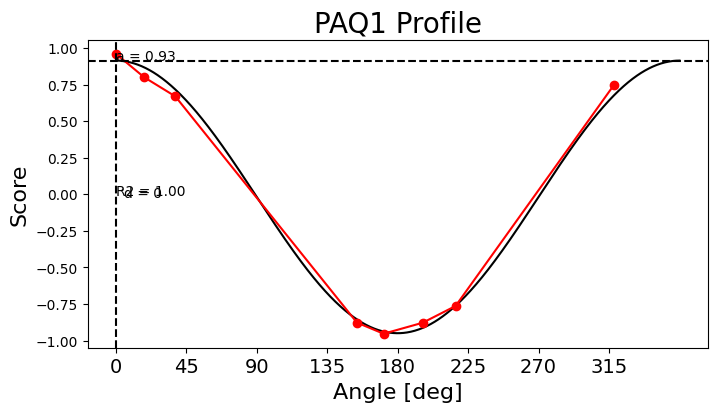
\includegraphics{Mitchell_Quasi-Circumplex_files/figure-latex/fig-profile-plots-output-1.png}

}

\subcaption{\label{fig-profile-plots-1}PAQ1}

\end{minipage}%
%
\begin{minipage}[t]{0.25\linewidth}

\centering{

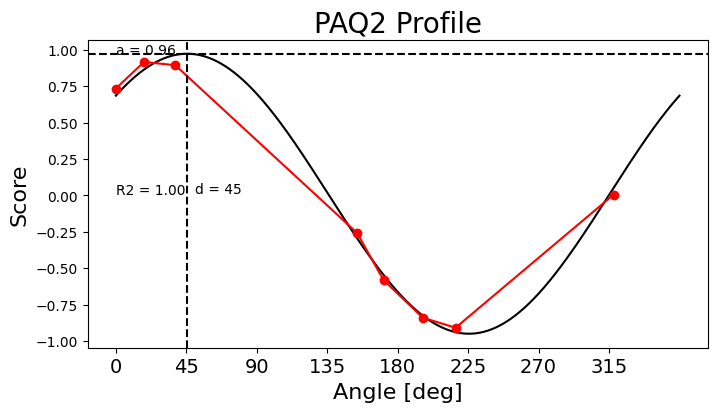
\includegraphics{Mitchell_Quasi-Circumplex_files/figure-latex/fig-profile-plots-output-2.png}

}

\subcaption{\label{fig-profile-plots-2}PAQ2}

\end{minipage}%
%
\begin{minipage}[t]{0.25\linewidth}

\centering{

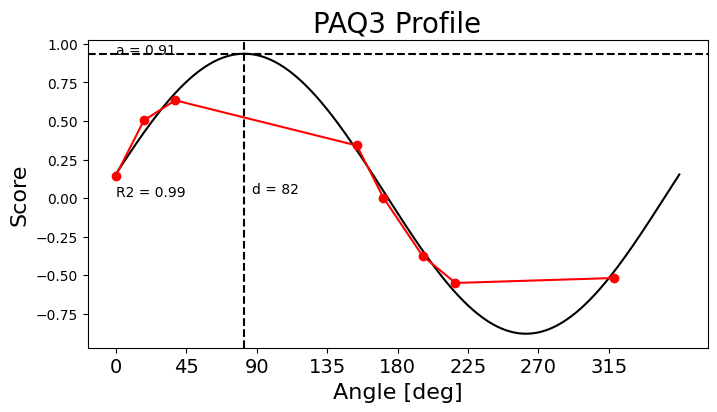
\includegraphics{Mitchell_Quasi-Circumplex_files/figure-latex/fig-profile-plots-output-3.png}

}

\subcaption{\label{fig-profile-plots-3}PAQ3}

\end{minipage}%
%
\begin{minipage}[t]{0.25\linewidth}

\centering{

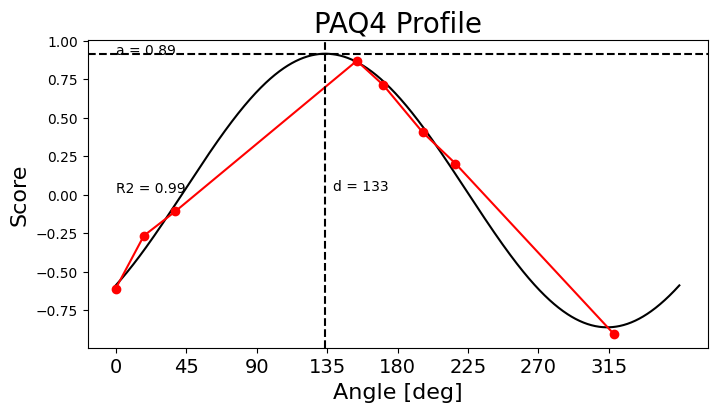
\includegraphics{Mitchell_Quasi-Circumplex_files/figure-latex/fig-profile-plots-output-4.png}

}

\subcaption{\label{fig-profile-plots-4}PAQ4}

\end{minipage}%
\newline
\begin{minipage}[t]{0.25\linewidth}

\centering{

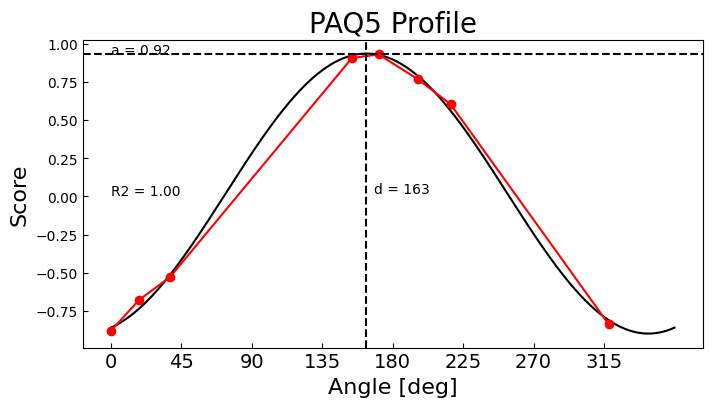
\includegraphics{Mitchell_Quasi-Circumplex_files/figure-latex/fig-profile-plots-output-5.png}

}

\subcaption{\label{fig-profile-plots-5}PAQ5}

\end{minipage}%
%
\begin{minipage}[t]{0.25\linewidth}

\centering{

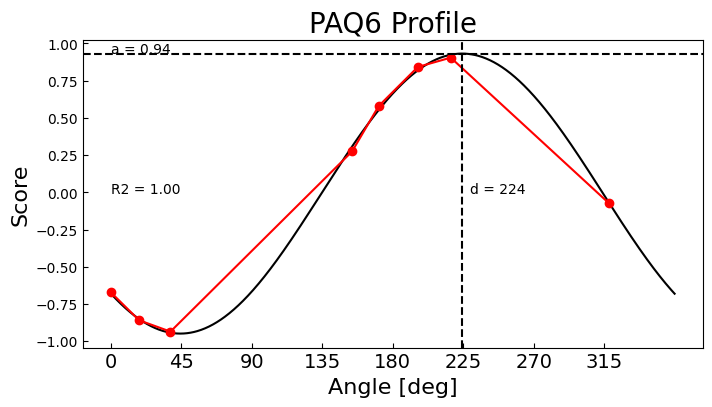
\includegraphics{Mitchell_Quasi-Circumplex_files/figure-latex/fig-profile-plots-output-6.png}

}

\subcaption{\label{fig-profile-plots-6}PAQ6}

\end{minipage}%
%
\begin{minipage}[t]{0.25\linewidth}

\centering{

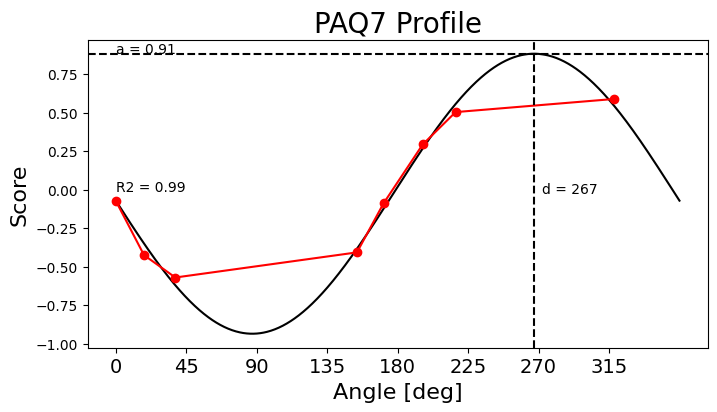
\includegraphics{Mitchell_Quasi-Circumplex_files/figure-latex/fig-profile-plots-output-7.png}

}

\subcaption{\label{fig-profile-plots-7}PAQ7}

\end{minipage}%
%
\begin{minipage}[t]{0.25\linewidth}

\centering{

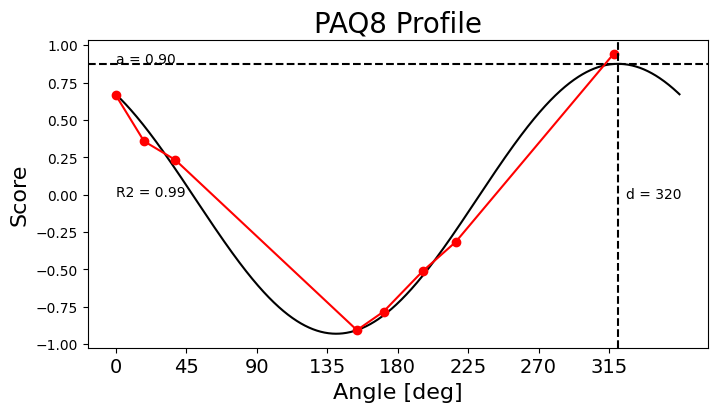
\includegraphics{Mitchell_Quasi-Circumplex_files/figure-latex/fig-profile-plots-output-8.png}

}

\subcaption{\label{fig-profile-plots-8}PAQ8}

\end{minipage}%

\caption{\label{fig-profile-plots}Profile plots for the Mandarin (cmn)
translation}

\end{figure}%

The model fit results for each translation are shown in
Table~\ref{tbl-corr-angles-fit}. Since every translation is able to
adequately locate the circumplex scales, we can proceed to the final
step of the analysis.

\begin{longtable}[]{@{}lllllllll@{}}

\caption{\label{tbl-corr-angles-fit}Fit results for locating the general
circumplex within each language}

\tabularnewline

\toprule\noalign{}
& PAQ1 & PAQ2 & PAQ3 & PAQ4 & PAQ5 & PAQ6 & PAQ7 & PAQ8 \\
\midrule\noalign{}
\endhead
\bottomrule\noalign{}
\endlastfoot
arb & 0.998 & 0.999 & 0.995 & 0.995 & 0.998 & 0.999 & 0.997 & 0.995 \\
cmn & 0.997 & 0.996 & 0.988 & 0.993 & 0.999 & 0.999 & 0.989 & 0.992 \\
deu & 0.998 & 0.999 & 0.999 & 0.998 & 0.998 & 0.998 & 0.999 & 0.998 \\
ell & 0.998 & 0.995 & 0.998 & 0.998 & 0.997 & 0.998 & 0.996 & 0.997 \\
eng & 0.997 & 0.998 & 0.999 & 0.996 & 0.997 & 0.999 & 0.998 & 0.994 \\
hrv & 0.997 & 0.997 & 0.994 & 0.995 & 0.997 & 0.998 & 0.995 & 0.991 \\
ind & 0.996 & 0.998 & 0.998 & 0.998 & 0.996 & 0.993 & 0.999 & 0.996 \\
ita & 0.892 & 0.996 & 0.998 & 0.986 & 0.980 & 0.991 & 0.996 & 0.977 \\
kor & 0.997 & 0.996 & 0.996 & 0.998 & 0.998 & 0.991 & 0.997 & 0.998 \\
nld & 0.993 & 0.999 & 0.999 & 0.998 & 0.998 & 0.996 & 0.999 & 0.999 \\
spa & 0.998 & 0.996 & 0.998 & 0.998 & 0.998 & 0.996 & 0.999 & 0.999 \\
swe & 0.994 & 0.998 & 0.997 & 0.997 & 0.996 & 0.997 & 0.997 & 0.996 \\
tur & 0.997 & 0.997 & 0.998 & 0.999 & 0.996 & 0.993 & 0.999 & 0.997 \\

\end{longtable}

\subsection{Step 4: Accurately locating circumplex items within each
language}\label{step-4-accurately-locating-circumplex-items-within-each-language-1}

Table~\ref{tbl-correspondence} shows the results of the congruence test
between the circumplex structure of the original instrument and the
circumplex structure of the translated instruments. In addition to
calculating these results with the adjusted angles to apply the Step 4
test, we also calculate the results using the unadjusted angles to
demonstrate the impact of the adjustment.

\begin{longtable}[]{@{}llllll@{}}

\caption{\label{tbl-correspondence}Correspondence between the general
circumplex and the language-specific circumplex}

\tabularnewline

\toprule\noalign{}
& Language & Eq Ang Model & Corr Ang Model & Eq Ang Procrustes & Corr
Ang Procrustes \\
\midrule\noalign{}
\endhead
\bottomrule\noalign{}
\endlastfoot
0 & arb & 0.992 & 0.943 & 0.982 & 0.982 \\
1 & cmn & 0.932 & 0.993 & 0.885 & 0.991 \\
2 & deu & 0.985 & 0.957 & 0.973 & 0.983 \\
3 & ell & 0.985 & 0.989 & 0.970 & 0.979 \\
4 & eng & 0.988 & 0.977 & 0.983 & 0.983 \\
5 & hrv & 0.990 & 0.969 & 0.982 & 0.985 \\
6 & ind & 0.965 & 0.951 & 0.935 & 0.982 \\
7 & ita & 0.984 & 0.952 & 0.974 & 0.975 \\
8 & kor & 0.958 & 0.977 & 0.921 & 0.975 \\
9 & nld & 0.978 & 0.972 & 0.939 & 0.978 \\
10 & spa & 0.986 & 0.981 & 0.967 & 0.978 \\
11 & swe & 0.986 & 0.973 & 0.972 & 0.976 \\
12 & tur & 0.957 & 0.986 & 0.921 & 0.980 \\

\end{longtable}

When the adjusted angles for each translation are applied, the resulting
circumplex scale location achieve good congruence with their theoretical
locations. It should be noted that this is not the case without using
the adjusted angles: locating the scales with the cmn translation using
the unadjusted angles results in a score of 0.885, below the fit
threshold of 0.9, but this increases to 0.991 when using the adjusted
angles (see Figure 6). All translations see some degree of improvement
by using the adjusted angles.

Figure~\ref{fig-cmn-correspondence} gives an example of the impact of
using the corrected angles for locating the circumplex scales.

\begin{figure}

\begin{minipage}[t]{0.50\linewidth}

\centering{

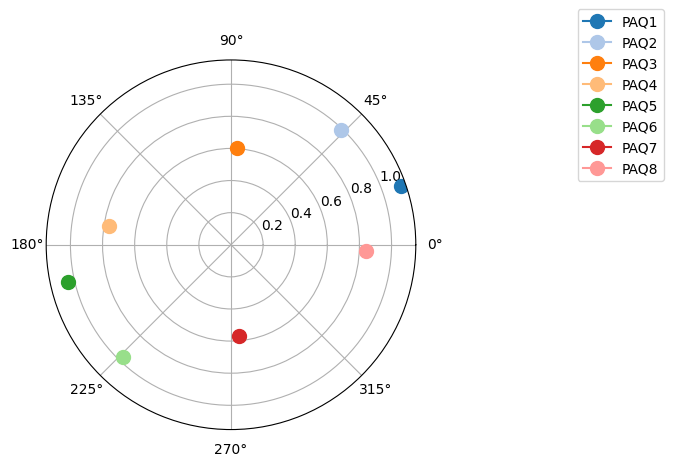
\includegraphics{Mitchell_Quasi-Circumplex_files/figure-latex/fig-cmn-correspondence-output-1.png}

}

\subcaption{\label{fig-cmn-correspondence-1}Equal angles}

\end{minipage}%
%
\begin{minipage}[t]{0.50\linewidth}

\centering{

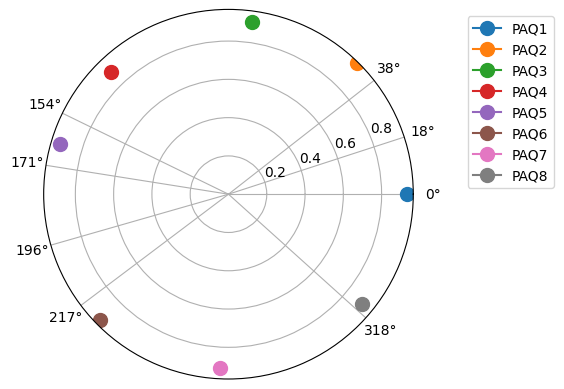
\includegraphics{Mitchell_Quasi-Circumplex_files/figure-latex/fig-cmn-correspondence-output-2.png}

}

\subcaption{\label{fig-cmn-correspondence-2}Corrected angles}

\end{minipage}%

\caption{\label{fig-cmn-correspondence}Locating the language-specific
circumplex for Mandarin, using equal angles and corrected angles}

\end{figure}%

\section*{Acknowledgements}\label{acknowledgements}
\addcontentsline{toc}{section}{Acknowledgements}

The authors would like to express their thanks to Karn Watcharasupat and
Steffen Lepa for their helpful discussions which contributed to the
development of this analysis procedure.


  \bibliography{FellowshipRefs.bib}


\end{document}
